\documentclass{dense_template}
\newcommand*{\name}{Felipe Alejandro Jiménez Castillo}
\newcommand*{\code}{215671386}
\newcommand*{\school}{Universidad de Guadalajara - CUCEI}
\newcommand*{\course}{Computación Tolerante a Fallas}
\newcommand*{\assignment}{Workflow}
\renewcommand{\contentsname}{Contenido}

\begin{document}
\maketitle
%%%%%%%%%%%%%%%%%%%%
\tableofcontents
\newpage
%%%%%%%%%%%%%%%%%%%%
\section{Introducción}
Un flujo de trabajo, también conocido como \textit{\textbf{workflow}} en inglés, es una secuencia de pasos y tareas interconectadas que se diseñan para lograr un objetivo específico. Los flujos de trabajo son comunes en una amplia variedad de entornos, desde negocios y organizaciones hasta procesos personales. Estos son algunos aspectos clave de los flujos de trabajo:
\begin{itemize}
    \item \textit{Secuencia de pasos}: Un flujo de trabajo se compone de una serie de pasos o tareas que se realizan en un orden particular. Cada paso puede depender del resultado del anterior.
    \item \textit{Automatización}: En muchos casos, los flujos de trabajo se diseñan para automatizar procesos y tareas, lo que puede aumentar la eficiencia y reducir la posibilidad de errores.
    \item \textit{Asignación de roles}: Los flujos de trabajo suelen incluir la asignación de tareas a elementos específicos. Esto asegura que cada parte del proceso se realice de manera adecuada.
    \item \textit{Reglas y condiciones}: Los flujos de trabajo a menudo incluyen reglas y condiciones que determinan cómo deben ejecutarse los pasos. Por ejemplo, una tarea puede estar programada para activarse solo después de que se cumpla cierta condición.
    \item \textit{Gestión y seguimiento}: Los flujos de trabajo suelen incluir herramientas para la gestión y seguimiento de tareas, lo que permite a los responsables supervisar el progreso y realizar ajustes según sea necesario.
\end{itemize}

%%%%%%%%%%%%%%%%%%%%
\section{Desarrollo}
\subsection{Script (\textit{python})}
Para el desarrollo de está actividad, se desarrollo un flujo de trabajo que trabajara con \textit{prefect}, de modo que, utilizando sus API's web, ver como es el proceso de trabajo en nuestro flujo de trabajo.

El programa está diseñado en 3 tareqas, de modo que nuestro flujo de trabajo este separado por partes y pueda ser modular:
\begin{enumerate}
    \item do\_request: Esta función realiza una petición a un API web que nos trae en formato JSON.
    \item do\_parse: Está función realiza el parseo de datos de texto plano a un formato JSON real.
    \item do\_print: Está función muestra los datos obtenidos por la petición.
\end{enumerate}

Con esto en mente se finalizo desarrollando una función que sería nuestro flujo principal y llamaría a las otras tareas para ser ejecutadas y demostradas.

 \begin{center}
    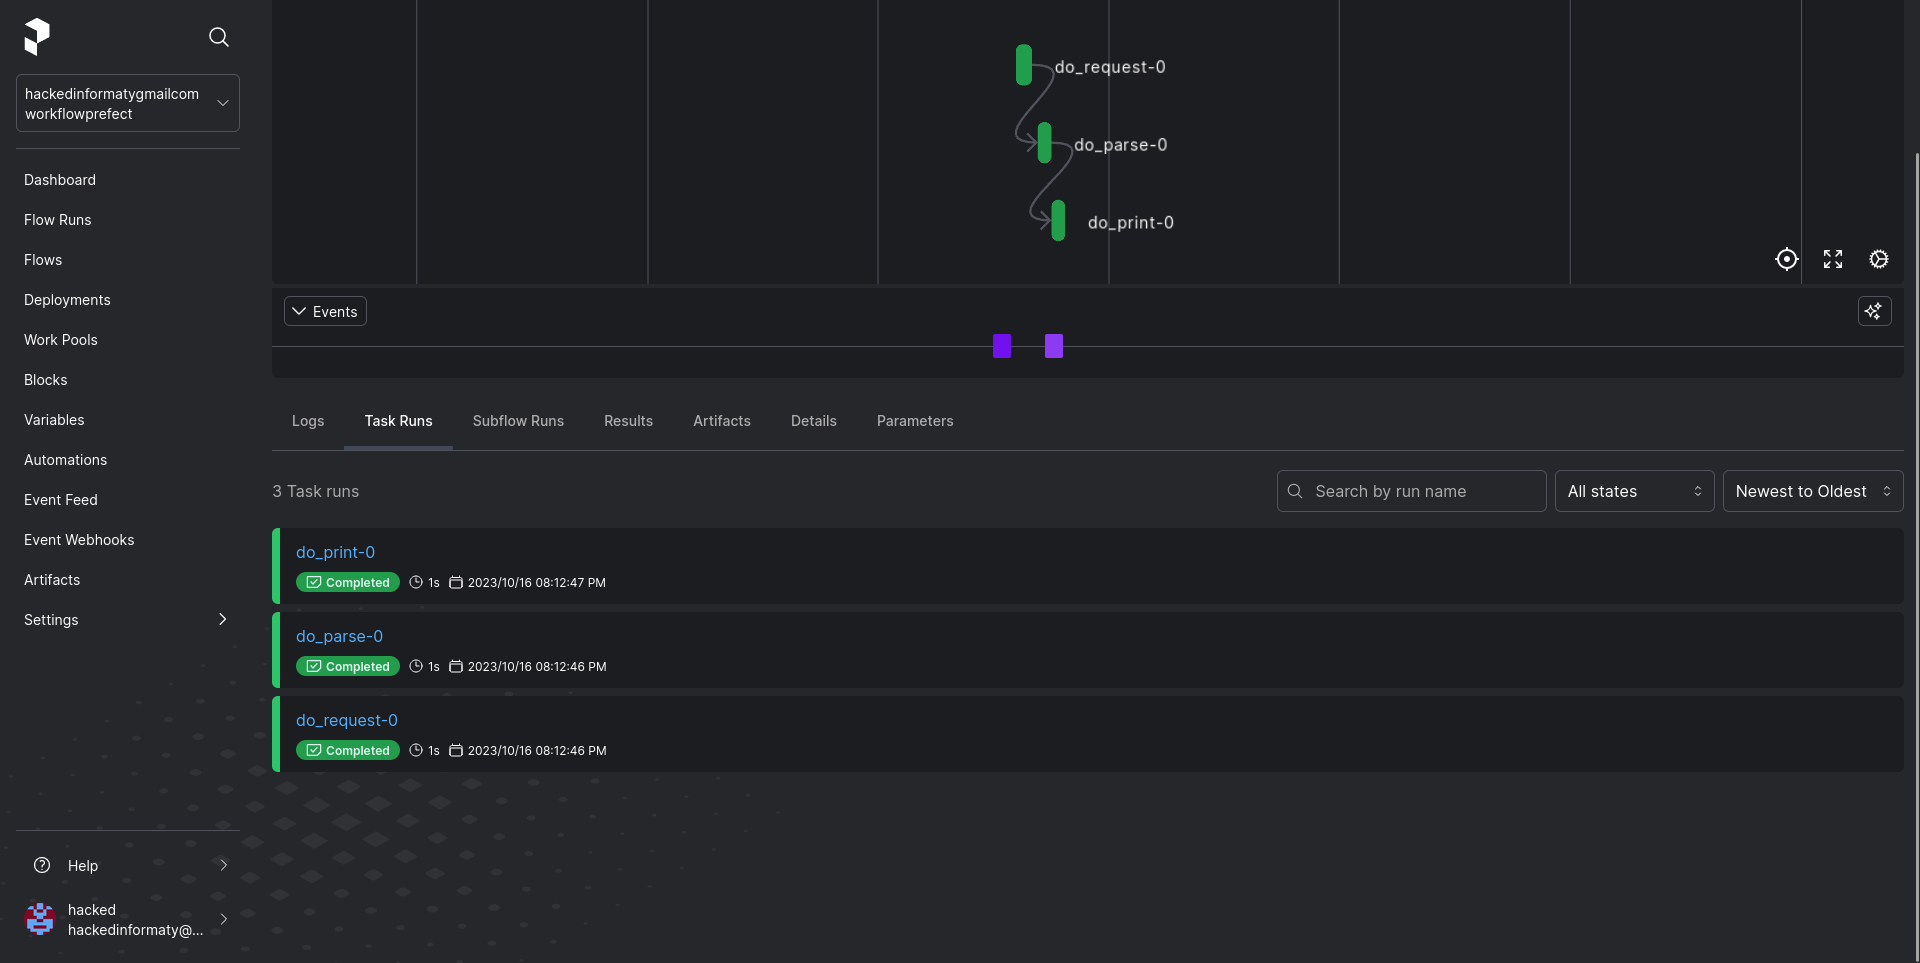
\includegraphics[width=0.9\textwidth]{1-workflow.png}
    \vspace{1cm}
    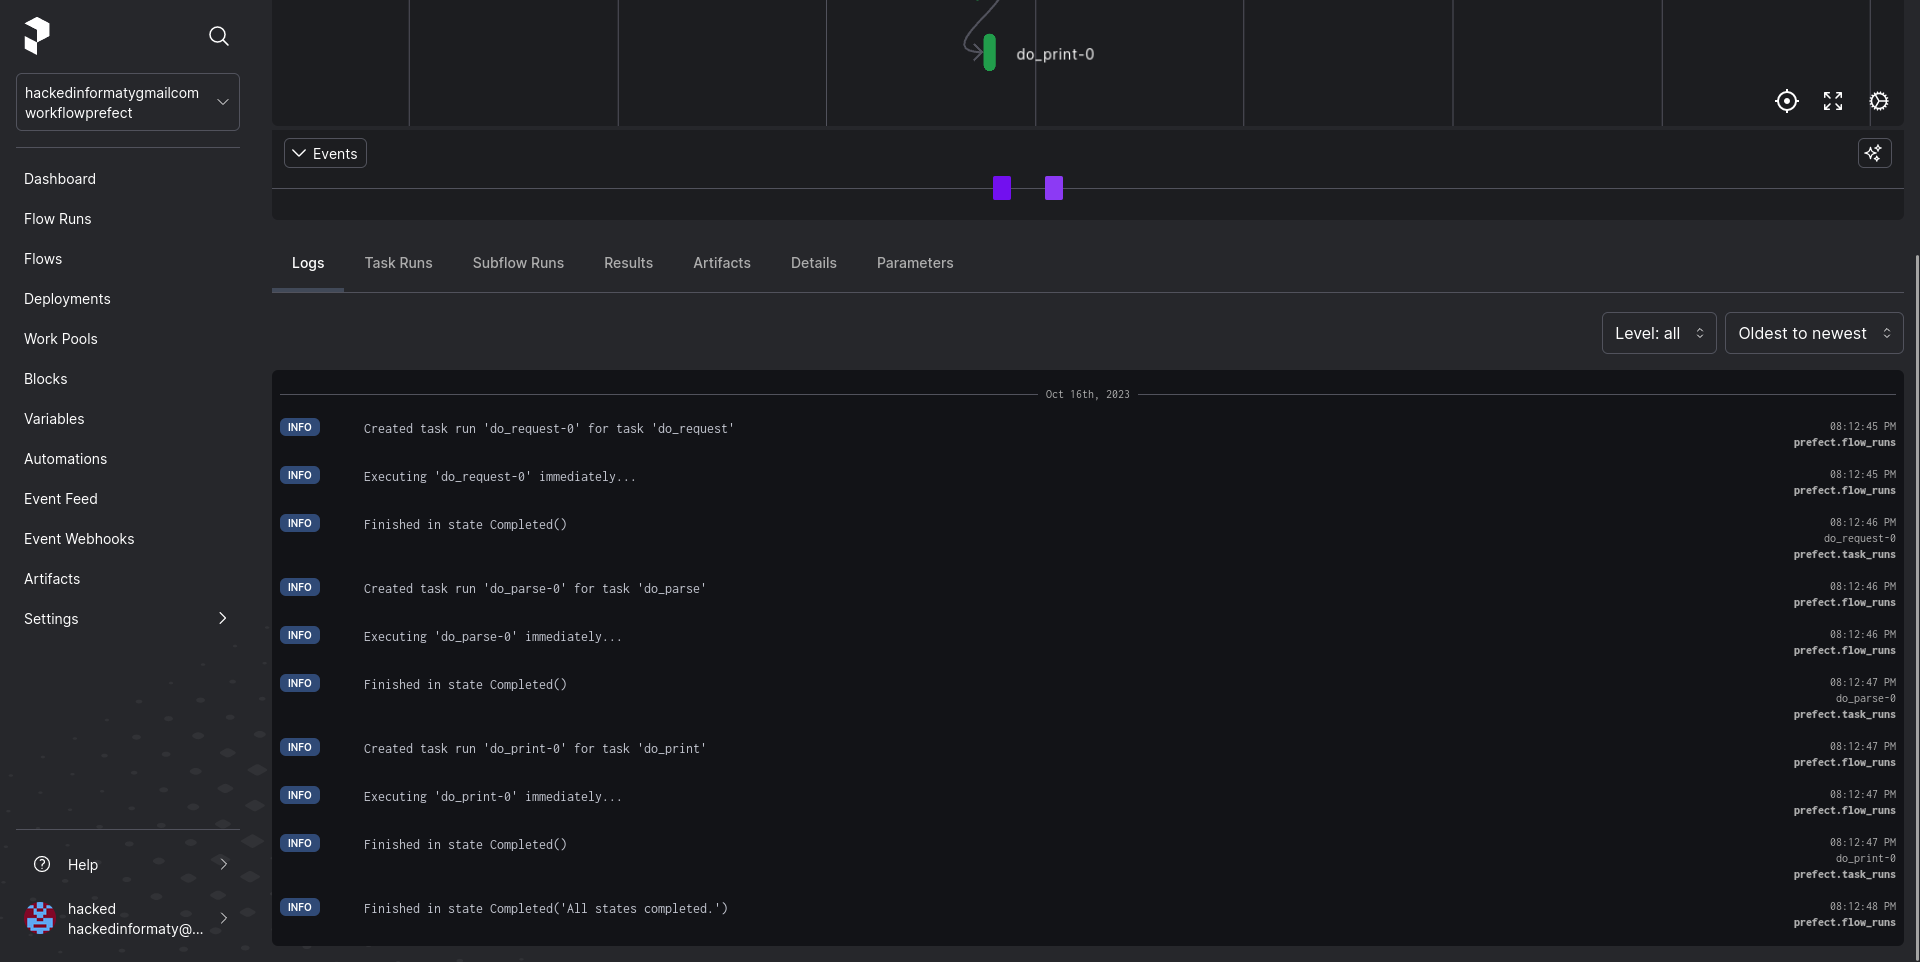
\includegraphics[width=0.9\textwidth]{2-workflow.png}
    \vspace{1cm}
    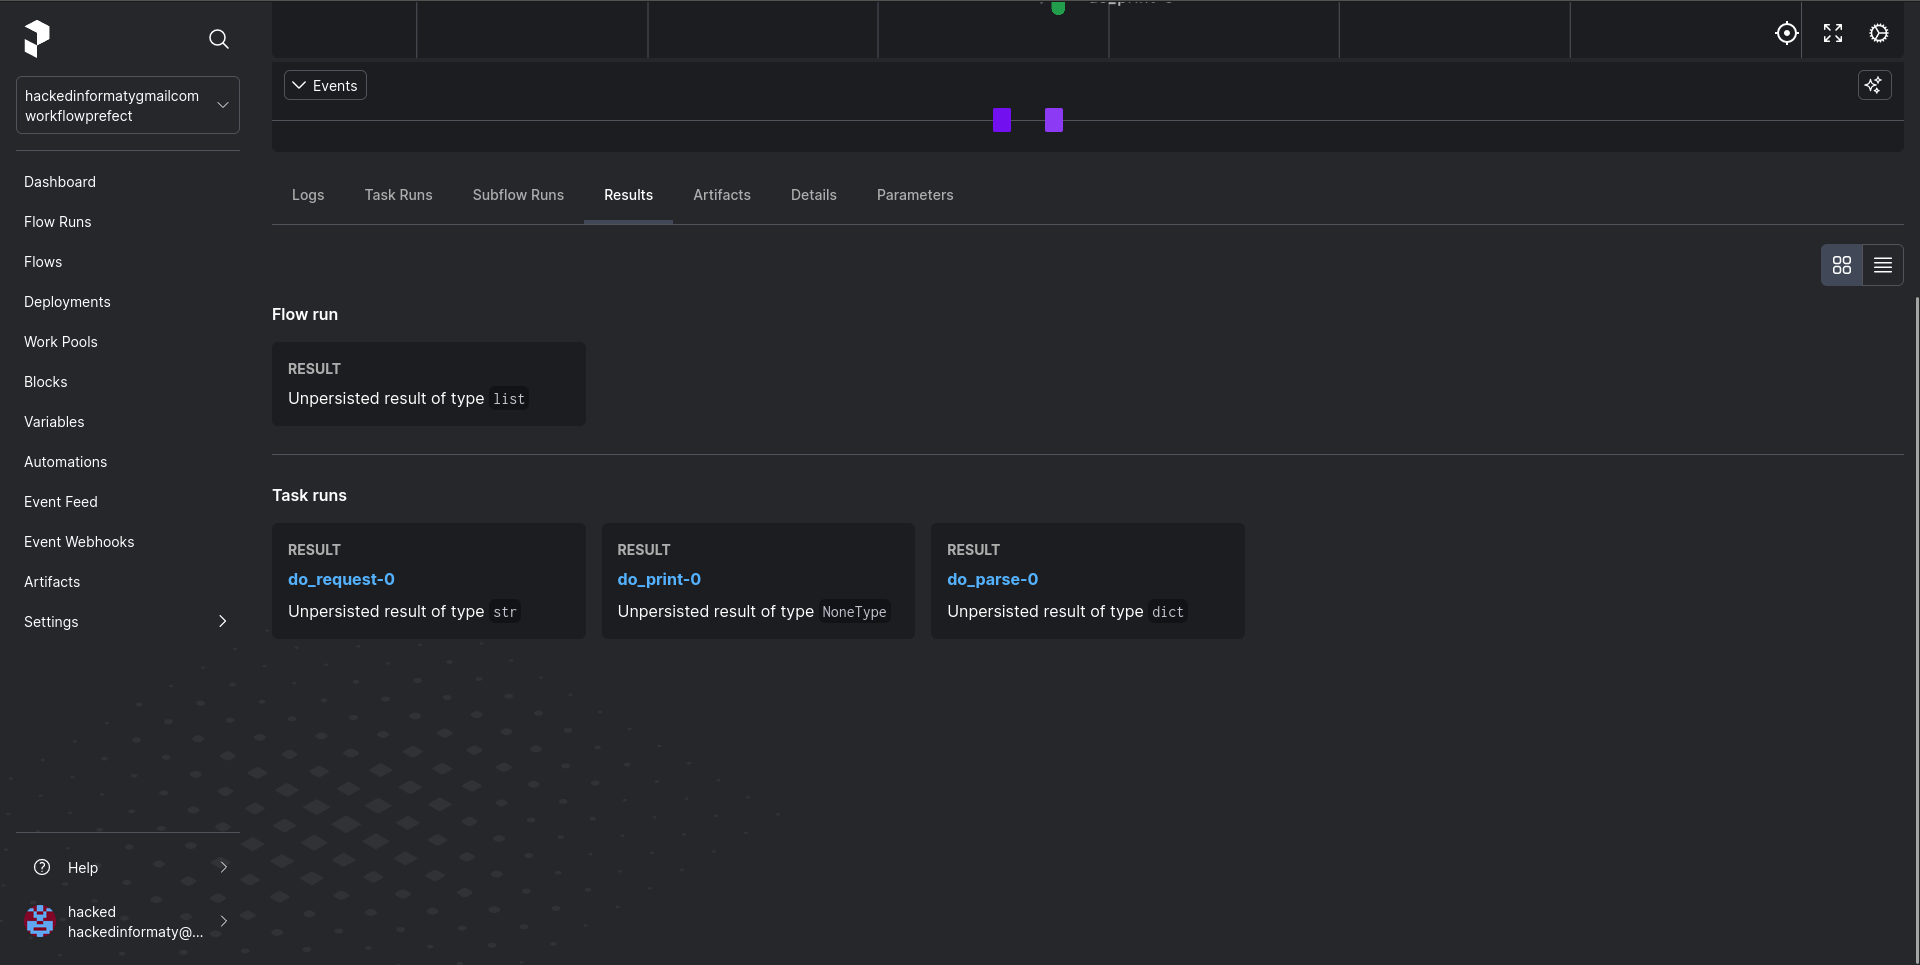
\includegraphics[width=0.9\textwidth]{3-workflow.png}
 \end{center}
%%%%%%%%%%%%%%%%%%%%
\pagebreak
%%%%%%%%%%%%%%%%%%%%
\section{Conclusión}
Los flujos de trabajo permiten automatizar tareas y procesos, lo que aumenta la eficiencia al eliminar la necesidad de realizar manualmente tareas repetitivas. Esto ahorra tiempo y recursos. Además al seguir un flujo de trabajo predefinido, se garantiza la consistencia en la ejecución de tareas. Esto es crucial en la producción de resultados confiables y de alta calidad. Por lo tanto en entornos empresariales y proyectos tecnológicos, los flujos de trabajo ayudan a gestionar la complejidad. Los proyectos suelen constar de muchas tareas interconectadas, y un flujo de trabajo claro y organizado facilita su gestión.

%%%%%%%%%%%%%%%%%%%%
\pagebreak
%%%%%%%%%%%%%%%%%%%%
\section{Bilbiografia}
\sloppy
\begin{enumerate}
    \item Sharp, A. (2008). Workflow modeling: Tools for process improvement and application development, second edition (2nd ed.). Artech House.
\end{enumerate}
\end{document}

